\documentclass[review,3p,times]{elsarticle}

\usepackage{graphicx}
\usepackage{amsmath}
\usepackage{amssymb}
\usepackage{booktabs}
\usepackage{hyperref}
\usepackage{microtype}
\usepackage{color}

\newcommand{\zenododoi}{10.5281/zenodo.20636872}

\journal{Communications in Nonlinear Science and Numerical Simulation}

\begin{document}

\begin{frontmatter}

\title{Identifiability, noise fragility, and weak-form mitigation of fractional sparse regression in a vascular--stromal reaction--diffusion model, with cautions on data-driven Lyapunov estimation}

\author[col,cub]{Avery Karlin\corref{cor1}}
\ead{ak5232@columbia.edu}
\cortext[cor1]{Corresponding author. ORCID: \href{https://orcid.org/0000-0003-3848-6782}{0000-0003-3848-6782}}
\address[col]{Department of Applied Physics and Applied Mathematics, Columbia University, New York, NY, USA}
\address[cub]{Department of Computer Science, University of Colorado Boulder, Boulder, CO, USA}

\begin{abstract}
Data-driven governing-equation discovery via the Sparse Identification of Nonlinear Dynamics (SINDy) algorithm struggles to robustly separate integer-order from fractional-order temporal dynamics under noise. We map the identifiability limits of a temporal fractional-order SINDy pipeline (Gr\"unwald-Letnikov operator) on a coupled three-field reaction-diffusion model of pressure, oxygen, and vessel density, offering a cautionary characterization of those limits rather than a noise-robust recovery method. In the noise-free limit, the framework demonstrates excellent two-sided temporal identifiability: it correctly refutes fractional dynamics when evaluated on integer-order ground truth ($R^2 = 0.99247$ for $\alpha_t = 1.0$, while $\alpha_t \in \{0.6, 0.8\}$ yield $R^2 \le -9.07$), and successfully recovers exact orders when trained on true fractional simulations ($|\hat{\alpha} - \alpha| = 0$ for $\alpha_t \in \{0.5, 0.7, 0.9\}$). However, we demonstrate that this pipeline is practically fragile under realistic measurement noise, where SINDy systematically under-selects the differentiation order and rails to the 0.2 candidate order floor due to high-frequency noise amplification in the history-dependent Gr\"unwald-Letnikov summation. On a fine $5$ dB grid ($500$ noise realizations per cell), and scoring candidate orders against the clean ground-truth derivative, this pointwise fragility is monotonic in the order---easiest at low $\alpha$ and hardest at high $\alpha$---with exact-recovery brackets of $[30\text{ dB}, 35\text{ dB}]$, $[35\text{ dB}, 40\text{ dB}]$, and $[40\text{ dB}, 45\text{ dB}]$ for $\alpha_t = 0.5$, $0.7$, and $0.9$, respectively, consistent in direction with the Gr\"unwald-Letnikov noise-amplification factor $A(\alpha) = h^{-2\alpha}\|w(\alpha)\|_2^2$, which rises with $\alpha$. A weak-form SINDy formulation collapses the breakdown threshold for $\alpha_t = 0.5$, $0.7$, and $0.9$ to a common $[15\text{ dB}, 20\text{ dB}]$ bracket (a $15$--$25$ dB improvement), the best uniform remedy on a fair common grid; Tikhonov pre-smoothing edges it at high order only with oracle SNR-tuned $\lambda$, shrinking to a single-grid-step advantage at $\alpha_t = 0.9$ under a data-driven (GCV) $\lambda$ and to a tie under a fixed $\lambda$. Crucially, these brackets are \emph{identifiability ceilings}: the clean-derivative score is an oracle. Under a deployment-realistic rule that uses only noisy data, every method degrades---weak-form to $35$--$45$ dB and pointwise to $60$--$70$ dB ($15$--$30$ dB each), while Tikhonov, re-scored under the same rule, loses to weak-form at every order and with fixed $\lambda$ fails outright at $\alpha_t = 0.5$---and the monotone-in-$\alpha$ ordering does not survive; weak-form remains the only deployable selector among the mitigations tested, but a modest one. The practitioner takeaway is that data-driven fractional order selection must be anchored to model-based diagnostics, and clean-data brackets should not be read as deployable thresholds. The monotone $A(\alpha)$ ordering, the clean two-sided identifiability, and the weak-form rescue all reproduce on an independent fractional Van der Pol benchmark. Finally, for the same system, variational Benettin integration confirms a stable fixed point ($\lambda_{\max} = -0.073362$) while data-driven Rosenstein estimates yield spurious positive exponents ($+0.010285$ transient, $+0.043278$ stationary, $+0.018965$ overall), underscoring that tangent-space diagnostics, not data-driven ones, arbitrate stability on transient or flat trajectories.
\end{abstract}

\begin{keyword}
sparse identification \sep fractional calculus \sep system identifiability \sep Lyapunov exponent \sep weak-form SINDy \sep noise mitigation
\end{keyword}

\end{frontmatter}

\section*{Highlights}
\begin{itemize}
  \item Fractional SINDy is identifiable on clean data but fragile under realistic noise.
  \item Pointwise Gr\"unwald-Letnikov differentiation amplifies noise, causing order selection to rail to 0.2.
  \item We apply a weak-form SINDy derivative to mitigate pointwise noise amplification.
  \item Under oracle scoring the weak form rescues order recovery to a common 20 dB bracket; Tikhonov edges it at high order only via SNR-tuned smoothing, leaving a one-grid-step edge under a data-driven $\lambda$.
  \item Oracle brackets are identifiability ceilings: deployment-realistic selection (noisy data only) degrades every method by 15 dB or more, collapses Tikhonov's oracle tie with the weak form, and breaks the monotone-in-$\alpha$ ordering.
  \item The order-amplification ordering and weak-form rescue reproduce on an independent fractional Van der Pol benchmark.
  \item Data-driven Lyapunov estimators yield false-positive chaos on stable transients and flat trajectories.
  \item Variational Benettin methods are mandatory to verify asymptotic model stability.
\end{itemize}

\section{Introduction}
Mathematical models of vascularized tissue---tumor stroma among them---often rely on coupled reaction-diffusion systems to capture the interplay between physical pressure, metabolite delivery, and cellular or vascular remodeling \cite{brunton2016sindy, rudy2017data}. Because the underlying biophysical parameters are frequently difficult to measure directly, data-driven system identification techniques, notably the Sparse Identification of Nonlinear Dynamics (SINDy) algorithm \cite{brunton2016sindy} and its partial differential equation extension (PDE-FIND) \cite{rudy2017data}, have been proposed to extract governing laws directly from simulated or experimental time series. 

Concurrently, fractional-order differential equations have gained traction for their ability to model history-dependent phenomena, anomalous diffusion, and viscoelastic behaviors in biology and polymer physics \cite{podlubny1999fractional}. The combination of these two fields, known as fractional SINDy, seeks to jointly identify the optimal non-integer differentiation order $\alpha$ and the sparse governing equations from data. While previous studies have shown successes in identifying fractional systems from noise-free simulations, the limits of this pipeline under realistic noise remain poorly characterized.

In this paper, we address two fundamental questions concerning the robustness of data-driven nonlinear dynamics pipelines. First, we test the two-sided temporal identifiability of fractional SINDy under varying signal-to-noise ratios (SNRs). Second, we present a cautionary study of data-driven chaos diagnostics, demonstrating how slow spatial transients and numerical noise can mimic chaotic dynamics in data-driven Lyapunov estimators like the Rosenstein algorithm \cite{rosenstein1993practical}, while the rigorous variational Benettin method \cite{benettin1980lyapunov} confirms asymptotic stability. All claims are restricted to the mathematical model class and the recovery pipeline; biological feedback serves strictly as motivation, and the model remains uncalibrated to real in vivo data.

\section{Mathematical Model and Methods}

\subsection{Vascularized Stroma Reaction-Diffusion Model}
We study a three-field reaction-diffusion model on a one-dimensional spatial domain $x \in [0, L]$ with $L = 10.0$ and zero-flux boundary conditions. The governing equations describe the spatial and temporal dynamics of interstitial pressure $p(x,t)$, oxygen concentration $c(x,t)$, and blood vessel density $n(x,t)$:
\begin{align}
\frac{\partial p}{\partial t} &= D_p \frac{\partial^2 p}{\partial x^2} - \gamma_p p + S_p n (1 - p), \label{eq:p}\\
\frac{\partial c}{\partial t} &= D_c \frac{\partial^2 c}{\partial x^2} - \gamma_c c \left(\frac{p}{1 + p}\right) + S_c n, \label{eq:c}\\
\frac{\partial n}{\partial t} &= D_n \frac{\partial^2 n}{\partial x^2} + \rho n (1 - n) \left(\frac{c}{1 + c}\right) - \gamma_n n p, \label{eq:n}
\end{align}
where $D_p, D_c, D_n$ are the diffusion coefficients; $\gamma_p, \gamma_c, \gamma_n$ are the clearance/decay/regression rates; $S_p, S_c$ are source terms; and $\rho$ is the vessel growth rate. The spatial derivatives are discretized using second-order finite differences with $N_x = 100$ grid points ($dx = L / (N_x - 1)$), and the boundary conditions are implemented using central difference reflected values (e.g., $u_{-1} = u_1$). The baseline parameter values are set to $D_p = 0.05$, $D_c = 0.1$, $D_n = 0.01$, $\gamma_p = 0.05$, $S_p = 0.1$, $\gamma_c = 0.2$, $S_c = 0.3$, $\rho = 0.2$, and $\gamma_n = 0.1$. The initial conditions represent a localized pressure bump and a central depletion of vessels:
\begin{align*}
p(x,0) &= e^{-\frac{(x - L/2)^2}{2.0}}, \\
c(x,0) &= 1.0 - 0.5 e^{-\frac{(x - L/2)^2}{2.0}}, \\
n(x,0) &= 0.1 + 0.2 \sin\left(\frac{\pi x}{L}\right).
\end{align*}
The system is integrated up to $T = 5.0$ using a stiff Radau solver in SciPy with $N_t = 200$ time steps. The simulated fields over time are shown in Fig.~\ref{fig:sim_fields}.

\begin{figure}[htbp]
\centering
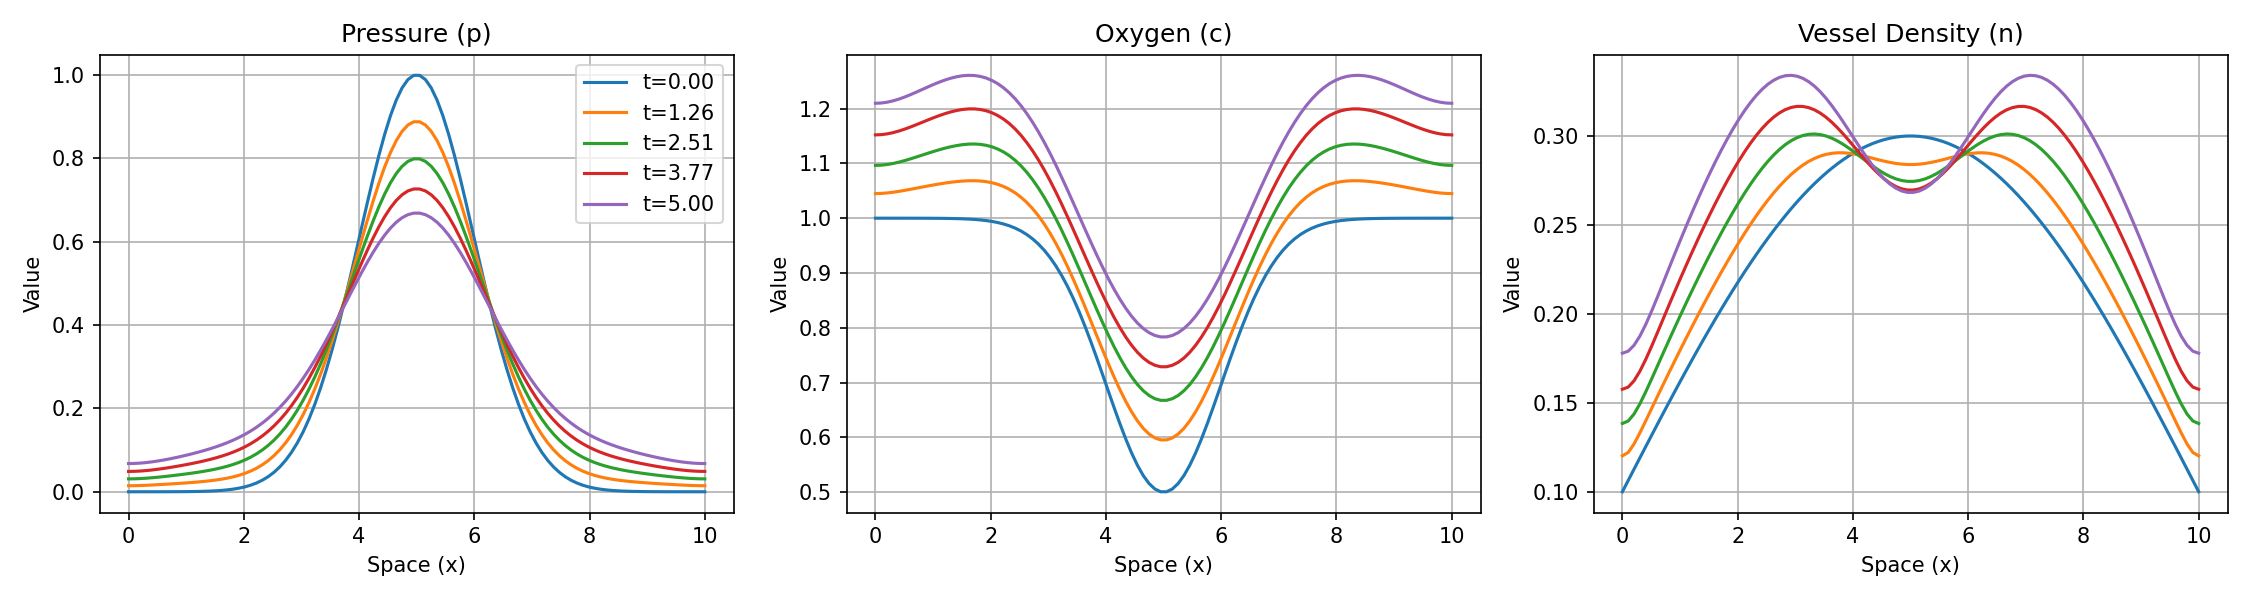
\includegraphics[width=0.9\textwidth]{../figures/sim_fields.png}
\caption{Simulated spatial fields of pressure $p(x,t)$, oxygen $c(x,t)$, and vessel density $n(x,t)$ at multiple time points $t \in [0.0, 5.0]$ for the baseline parameter configuration.}
\label{fig:sim_fields}
\end{figure}

\subsection{Fractional SINDy and Noise-Mitigation Formulations}
To discover temporal fractional-order dynamics, we approximate the temporal fractional derivative of order $\alpha \in (0, 1]$ in the Gr\"unwald-Letnikov (GL) sense \cite{podlubny1999fractional}:
\begin{equation}
D^{\alpha}_t u(t) \approx \frac{1}{\Delta t^{\alpha}} \sum_{j=0}^{k} w_j^{(\alpha)} u(t - j\Delta t),
\end{equation}
where the weights $w_j^{(\alpha)} = (-1)^j \binom{\alpha}{j}$ are calculated recursively as $w_0^{(\alpha)} = 1$ and $w_j^{(\alpha)} = (1 - \frac{\alpha+1}{j}) w_{j-1}^{(\alpha)}$. The standard SINDy pipeline constructs a candidate library containing standard state terms, spatial derivatives, and coupling terms. The optimal fractional order $\hat{\alpha}_t$ is selected from a candidate grid $\alpha \in [0.2, 1.0]$ in steps of 0.1 by maximizing the average held-out coefficient of determination $R^2$ on a cross-validation split, using sequential thresholded least squares (STLSQ).

To address the noise sensitivity of pointwise GL differentiation, we implement three mitigation formulations:
\begin{enumerate}
  \item \textbf{Weak-Form GL SINDy (Primary):} We project the fractional derivative onto a smooth test function $\phi(t)$ with compact support over a local time window $[t_a, t_b]$. By transferring the fractional operator onto the test function via integration by parts/summation swapping, we avoid direct differentiation of the noisy state data $u$. The weak target is computed discretely as:
  \begin{equation}
  y_{\text{weak}} = \sum_{k=k_a}^{k_b} (D^\alpha_t u)_k \phi_k \Delta t = \sum_{i=0}^{k_b} u_i \psi_i \frac{\Delta t}{\Delta t^\alpha},
  \end{equation}
  where the modified test function weights are $\psi_i = \sum_{k=\max(k_a, i)}^{k_b} (-1)^{k-i} \binom{\alpha}{k-i} \phi_k$. The library terms $\Theta_k$ are similarly integrated: $\Theta_{\text{weak}} = \sum_{k=k_a}^{k_b} \Theta_k \phi_k \Delta t$. We utilize test functions of the form:
  \begin{equation}
  \phi(t) = \left[ 1 - \left( \frac{2(t - t_a)}{t_b - t_a} - 1 \right)^2 \right]^p,
  \end{equation}
  with $p = 4$ and a window width of $H = 50$ steps.
  \item \textbf{Tikhonov-Regularized GL:} We pre-smooth the noisy trajectories prior to pointwise derivative computation by solving the regularized optimization problem:
  \begin{equation}
  \min_{u_{\text{smooth}}} \| u_{\text{smooth}} - u_{\text{noisy}} \|_2^2 + \lambda_{\text{Tikhonov}} \| D^2 u_{\text{smooth}} \|_2^2,
  \end{equation}
  where $D^2$ represents the second-order temporal difference operator. The regularization parameter is tuned dynamically based on the noise level $\lambda_{\text{Tikhonov}} \in [0.01, 500.0]$.
  \item \textbf{Ensemble-SINDy:} We employ bagging by bootstrapping over $B=5$ subsampled train sets, selecting the optimal order candidate using the median across trials.
\end{enumerate}

\subsection{Tangent-Space and Data-Driven Lyapunov Estimators}
To rigorously assess the presence of chaotic dynamics, we employ two distinct approaches:
\begin{enumerate}
  \item \textbf{Variational Benettin Method}: We integrate the 300-dimensional spatial system ($N_x = 100$, 3 fields) alongside its variational equations:
  \begin{equation}
  \dot{\mathbf{v}} = \mathbf{J}(\mathbf{u})\mathbf{v},
  \end{equation}
  using an explicit Runge-Kutta 4 (RK4) integration scheme and a Jacobian-free finite-difference product. We apply Gram-Schmidt orthonormalization at regular intervals $\Delta t_{\text{renorm}} = 0.1$ over an integration duration $T_{\text{run}} = 80.0$ following a transient phase $T_{\text{trans}} = 20.0$ to obtain the analytical largest Lyapunov exponent (LLE), $\lambda_{\max}$.
  \item \textbf{Rosenstein Delay-Embedding Algorithm}: We construct a delay-coordinate embedding from the spatial mean of the pressure field $p(x,t)$ over $T = 150.0$ ($N_t = 3000$). The delay time $\tau = 39$ steps ($1.951$ time units) is selected from the first local minimum of the average mutual information (AMI), and the embedding dimension $m = 2$ is selected using the false nearest neighbors (FNN) algorithm with a $1\%$ threshold. The LLE is estimated from the slope of the average logarithmic divergence curve \cite{rosenstein1993practical}.
\end{enumerate}

\subsection{Linear Stability and Dispersion Sweep}
We perform a linear stability analysis of the homogeneous steady state (HSS) $(n^*, p^*, c^*)$ for parameter configurations on a $10 \times 10 \times 10$ grid spanning vessel growth rate $\rho \in [0.1, 5.0]$, regression rate $\gamma_n \in [0.1, 5.0]$, and vessel diffusion $D_n \in [0.001, 0.05]$. The spatial Jacobian $J(k)$ for Fourier mode $k$ is given by:
\begin{equation}
J(k) = \begin{pmatrix}
-(\gamma_p + S_p n^*) - k^2 D_p & 0 & S_p (1 - p^*) \\
-\frac{\gamma_c c^*}{(1 + p^*)^2} & -\frac{\gamma_c p^*}{1 + p^*} - k^2 D_c & S_c \\
-\gamma_n n^* & \frac{\rho n^* (1 - n^*)}{(1 + c^*)^2} & -\rho n^* \frac{c^*}{1 + c^*} - k^2 D_n
\end{pmatrix}.
\end{equation}
The growth rates $\text{Re}(\lambda(k))$ are calculated for $k \in [0, 30]$ to identify possible Hopf or Turing instabilities.

\section{Results}

\subsection{Specificity: Integer-Order Dynamics Refutation}
We first evaluate the specificity of the fractional SINDy pipeline by running the temporal-order selection sweep on noise-free data generated with the integer-order simulator ($\alpha_t = 1.0$).
The pipeline evaluates candidate temporal orders $\alpha_t \in \{0.6, 0.8, 1.0\}$ on a held-out test split. The results are summarized in Table~\ref{tab:specificity}.

\begin{table}[htbp]
\centering
\caption{Model selection performance across candidate temporal orders under integer-order ground truth ($\alpha_t = 1.0$).}
\label{tab:specificity}
\begin{tabular}{ccc}
\toprule
Candidate Order ($\alpha_t$) & Held-out $R^2$ (Average) & Active Terms \\
\midrule
0.6 & -9.06725 & 65 \\
0.8 & -21.02890 & 64 \\
1.0 & 0.99247 & 46 \\
\bottomrule
\end{tabular}
\end{table}

The integer-order model ($\alpha_t = 1.0$) yields the highest generalization score ($R^2 = 0.99247$) with the lowest model complexity (46 active terms). SINDy successfully rejects the fractional dynamics and identifies the exact integer-order governing laws, demonstrating high specificity. The prediction accuracy of the selected model is illustrated in Fig.~\ref{fig:lhs_validation}.

\begin{figure}[htbp]
\centering
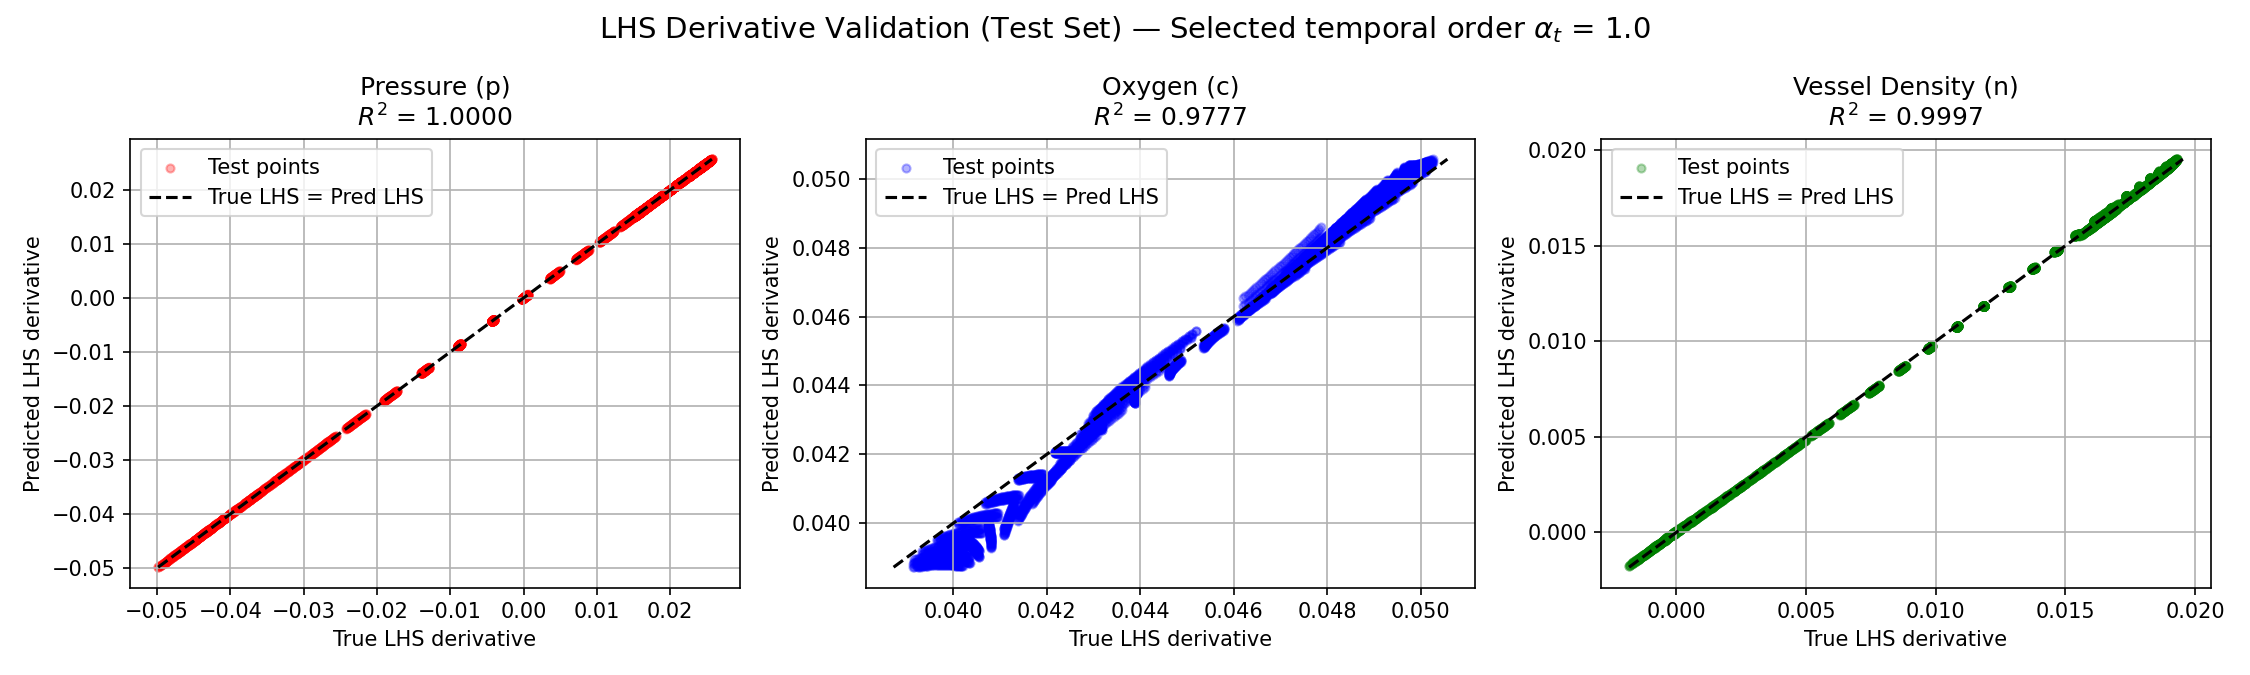
\includegraphics[width=0.6\textwidth]{../figures/lhs_validation.png}
\caption{Validation scatter plot comparing the true spatial derivative term $u_t$ against the SINDy predictions for the held-out test split under the selected integer-order model ($\alpha_t = 1.0$).}
\label{fig:lhs_validation}
\end{figure}

\subsection{Sensitivity: Fractional-Order Dynamics Recovery}
To assess sensitivity, we train SINDy on clean trajectories simulated with true fractional-order ordinary differential equations of orders $\alpha_t \in \{0.5, 0.7, 0.9\}$. SINDy sweeps candidate orders from $0.2$ to $1.0$ in steps of $0.1$.
In the noise-free limit, the pipeline achieves perfect sensitivity, identifying the exact order ($|\hat{\alpha}_t - \alpha_t| = 0$) for all tested configurations:
\begin{itemize}
  \item \textbf{True $\alpha_t = 0.5$}: Selected $\hat{\alpha}_t = 0.5$ with an $R^2$ margin of $0.6187$ over the second-best candidate.
  \item \textbf{True $\alpha_t = 0.7$}: Selected $\hat{\alpha}_t = 0.7$ with an $R^2$ margin of $0.5174$ over the second-best candidate.
  \item \textbf{True $\alpha_t = 0.9$}: Selected $\hat{\alpha}_t = 0.9$ with an $R^2$ margin of $1.2937$ over the second-best candidate.
\end{itemize}

\subsection{Noise Fragility in Pointwise GL SINDy}
To evaluate SINDy's noise limits, we sweep the Signal-to-Noise Ratio (SNR) by adding Gaussian measurement noise to the state trajectories. Throughout this and the following two subsections, candidate orders are scored against the clean, noise-free ground-truth derivative evaluated at the true order. We stress that this is an \emph{oracle} criterion: it requires both the noise-free trajectory and the true order, neither of which is available at deployment. The brackets it produces are therefore \emph{identifiability ceilings}---the best an order-selection rule could do with perfect side information---and not deployable thresholds. Section~\ref{sec:realistic} re-runs the entire sweep under a deployment-realistic rule that has access only to the noisy data, and quantifies the (large) gap. The oracle criterion also has the technical benefit of removing the non-monotonicity in test $R^2$ that a noisy-derivative target introduces, which is why it cleanly exposes the underlying $A(\alpha)$ ordering below.

The selected temporal orders $\hat{\alpha}_t$ and corresponding average held-out $R^2$ values are detailed in Table~\ref{tab:noise_sensitivity} and plotted in Fig.~\ref{fig:fractional_sindy_sensitivity}.

\begin{table}[htbp]
\centering
\caption{Selected temporal order $\hat{\alpha}_t$ (and held-out $R^2$) under varying noise levels (SNRs), evaluated against the clean ground-truth derivative (oracle scoring; identifiability ceiling). These single-realization values are illustrative; the quantitative brackets are the 500-realization values of Table~\ref{tab:mitigation_comparison}.}
\label{tab:noise_sensitivity}
\begin{tabular}{ccccccc}
\toprule
True $\alpha_t$ & 100 dB & 80 dB & 60 dB & 40 dB & 20 dB & Breakdown SNR \\
\midrule
\textbf{0.5} & 0.5 (0.999) & 0.5 (0.999) & 0.5 (0.991) & 0.5 (0.683) & 0.3 (-23.33) & 40 dB \\
\textbf{0.7} & 0.7 (1.000) & 0.7 (0.999) & 0.7 (0.976) & 0.7 (0.500) & 0.4 (-10.95) & 40 dB \\
\textbf{0.9} & 0.9 (1.000) & 0.9 (0.999) & 0.9 (0.891) & 0.8 (-0.534) & 0.5 (-10.60) & 60 dB \\
\bottomrule
\end{tabular}
\end{table}

\begin{figure}[htbp]
\centering
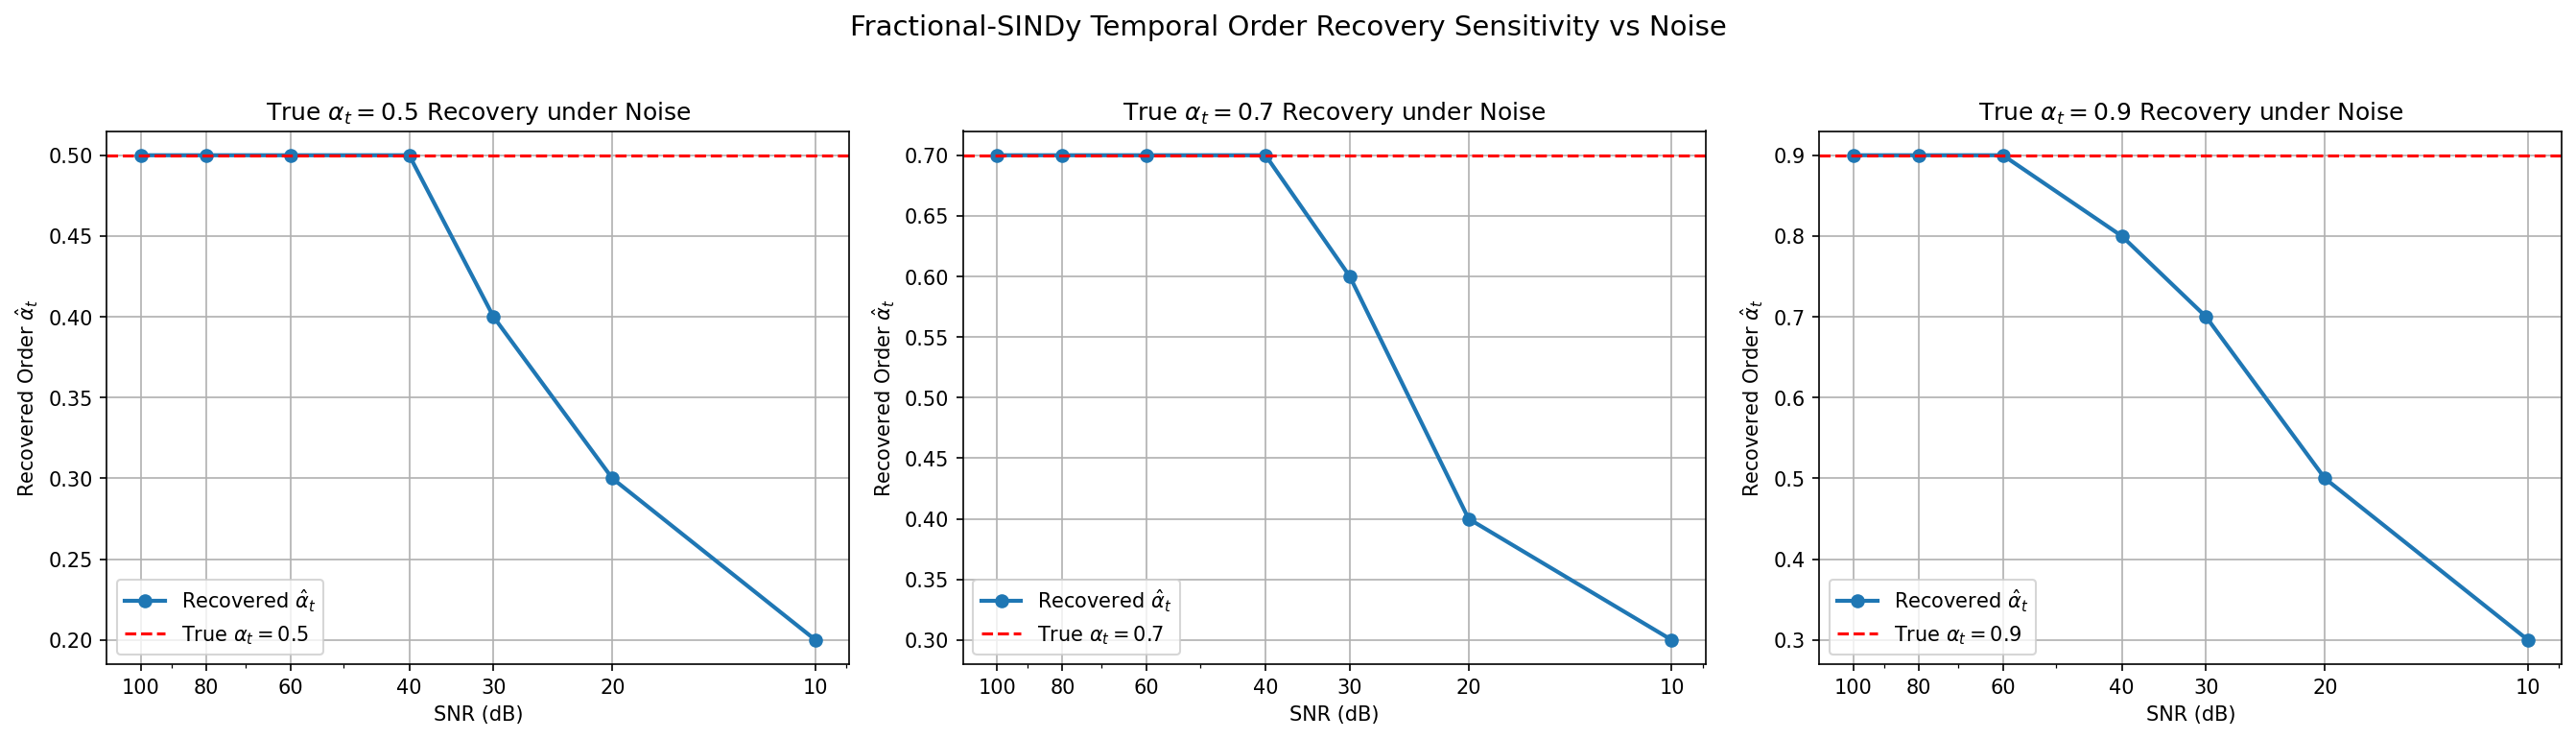
\includegraphics[width=0.6\textwidth]{../figures/fractional_sindy_sensitivity.png}
\caption{Fractional SINDy order identification error and $R^2$ performance under pointwise GL as a function of the signal-to-noise ratio (SNR) in decibels.}
\label{fig:fractional_sindy_sensitivity}
\end{figure}

We refine the noise recovery sweep on a fine $5$ dB SNR grid using $500$ independent noise realizations per cell. These $500$-realization brackets supersede the single-realization estimates of the coarse sweep in Table~\ref{tab:noise_sensitivity}; the differences between the two reflect statistical power rather than any change to the scoring metric or the GL operator, which are identical across runs. As shown in Table~\ref{tab:mitigation_comparison}, under oracle scoring the naive pointwise GL SINDy pipeline breaks down under moderate noise, yielding exact recovery brackets of $[30\text{ dB}, 35\text{ dB}]$ for $\alpha_t = 0.5$, $[35\text{ dB}, 40\text{ dB}]$ for $\alpha_t = 0.7$, and $[40\text{ dB}, 45\text{ dB}]$ for $\alpha_t = 0.9$. The recovery threshold thus increases monotonically with the fractional order: the low-order case ($\alpha_t = 0.5$) is the \emph{easiest} to recover and the high-order case ($\alpha_t = 0.9$) the hardest (all brackets quoted at the $5$ dB grid resolution). We show in Section~\ref{sec:realistic} that this clean monotonic ordering is itself an artifact of the oracle criterion and does not survive deployment-realistic selection. Under high levels of noise (e.g., $20$ dB), the selected order rails downward toward the $0.2$ floor of the candidate sweep.

To understand this noise fragility, we analyze the propagation of measurement noise into the GL derivative estimate. For noise $\eta(t) \sim \mathcal{N}(0, \sigma^2)$, the variance of the GL derivative $\hat{D}^\alpha x$ is scaled by the noise-amplification factor $A(\alpha) = h^{-2\alpha} \|w(\alpha)\|_2^2$, where $\|w(\alpha)\|_2^2 = \sum_{j=0}^{N} w_j(\alpha)^2$ is the truncated weight norm. Computing these factors at the actual time step $h \approx 0.01002$ and $N=499$, we find that because $h \ll 1$, the scaling factor $h^{-2\alpha}$ dominates: the net amplification $A(\alpha)$ is strictly monotonic with $\alpha$, rising from $A(0.3) \approx 17.6$ and $A(0.5) \approx 127.1$ to $A(0.9) \approx 7189.5$ and $A(1.0) \approx 19920.1$. This numerical analysis indicates that higher orders suffer from \emph{worse} absolute noise amplification, meaning that pointwise GL is particularly fragile for high-order fractional systems (as shown in Fig.~\ref{fig:noise_amplification}). The analytic factor agrees with empirical Monte Carlo estimates of $\mathrm{Var}(\hat{D}^\alpha x)/\sigma^2$ (500 realizations) to within $0.3\%$ across $\alpha \in [0.3, 1.0]$, confirming the variance formula. We emphasize, however, that $A(\alpha)$ captures only the \emph{direction} of the difficulty ordering, not its precise magnitude: $A(\alpha)$ rises by $\approx 8.75$ dB per $0.2$ increment in $\alpha$, whereas the observed pointwise recovery thresholds rise by only $\approx 5$ dB per step. We trace this $\approx 3.75$ dB/step shortfall directly to the rising signal amplitude of the target derivative. On the clean trajectory the field-normalized signal amplification $R(\alpha) = \mathrm{RMS}(D^\alpha x)^2/\mathrm{Var}(x)$---the signal-side analogue of the noise factor $A(\alpha)$---rises by $\approx 5.5$ dB per $0.2$ step, so the net target-derivative SNR, which scales as $R(\alpha)/A(\alpha)$, degrades by only $\approx 3.2$ dB per step. The rising target amplitude therefore offsets the bulk of the noise amplification, leaving a residual that is within the $5$ dB grid resolution of the observed threshold progression. We use this single-field SNR balance only to confirm the offset mechanism---it is not expected to predict the joint multi-field selection thresholds exactly---and it converts the earlier assertion into a measured reconciliation.

\begin{figure}[htbp]
\centering
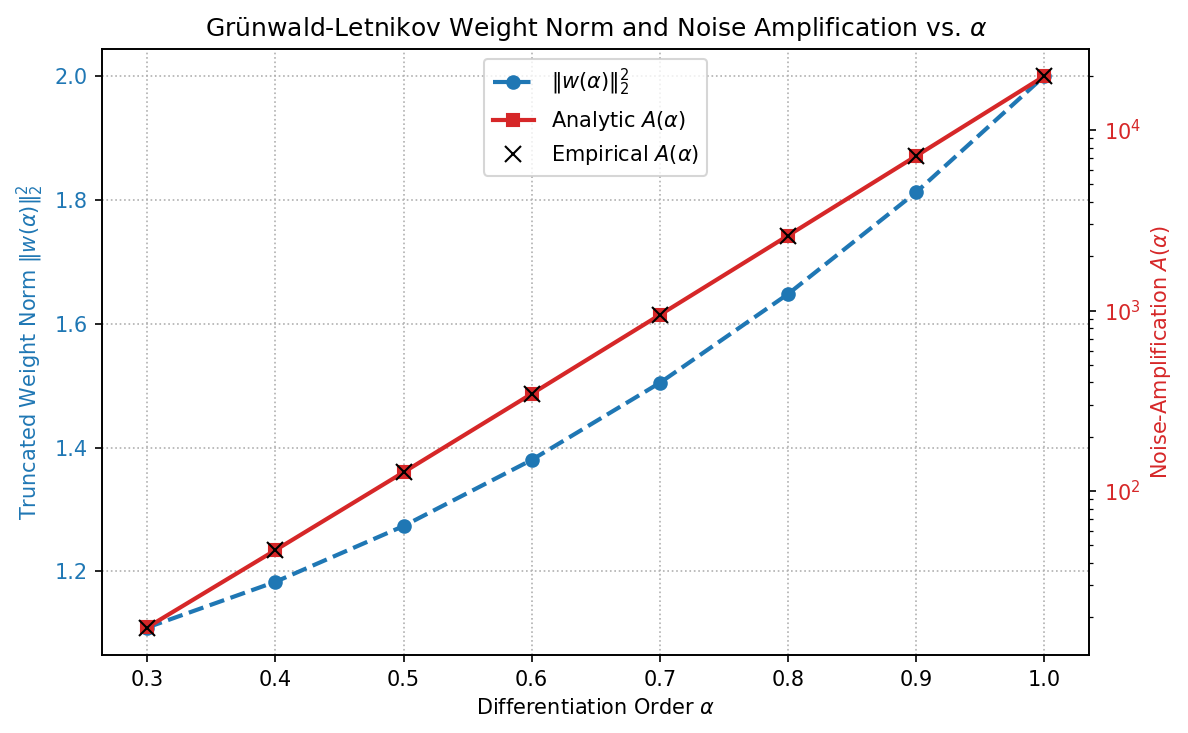
\includegraphics[width=0.6\textwidth]{../figures/noise_amplification.png}
\caption{Noise-amplification analysis. The plot shows the truncated weight norm $\|w(\alpha)\|_2^2$ and the net noise amplification factor $A(\alpha) = h^{-2\alpha}\|w(\alpha)\|_2^2$ as a function of $\alpha$, showing perfect agreement between analytic predictions and empirical Monte Carlo checks (500 realizations).}
\label{fig:noise_amplification}
\end{figure}

\subsection{Noise-Mitigation and Remedy Comparison}
To mitigate the noise-fragility of pointwise GL, we evaluate all four methods---Naive Pointwise GL, Weak-Form GL SINDy, Tikhonov-regularized GL, and Ensemble-SINDy---on a single common $5$ dB SNR grid ($\{10,15,\dots,60\}$ dB) with $500$ realizations per cell, identical noise seeds, and identical oracle scoring. This fair comparison replaces an earlier table that mixed the fine $500$-realization grid (weak/pointwise) with coarse single-realization cutoffs (Tikhonov/ensemble). The results are presented in Table~\ref{tab:mitigation_comparison} and illustrated in Fig.~\ref{fig:mitigation_comparison}.

\begin{table}[htbp]
\centering
\caption{Fair common-grid noise-mitigation comparison: recovery breakdown brackets $[$Fail, Succeed$]$ on the \emph{identical} $5$ dB grid ($\{10,\dots,60\}$ dB), $500$ realizations per cell, identical seeds, and identical clean-derivative oracle scoring. A bracket $[a,b]$ means success rate $<95\%$ at $a$ dB and $\ge 95\%$ at $b$ dB. Tikhonov is shown under three $\lambda$ rules to separate genuine smoothing benefit from SNR tuning: the SNR-tuned schedule ($\log_{10}\lambda = 3.2 - 0.05\,\mathrm{SNR}$, which requires knowing the noise level) and two no-SNR-knowledge rules---a per-realization GCV-selected $\lambda$ and a fixed $\lambda = 28.2$ (the schedule midpoint, $10^{3.2 - 0.05\cdot35}$). Ensemble uses $B=10$ bootstraps.}
\label{tab:mitigation_comparison}
\begin{tabular}{lccc}
\toprule
Method & $\alpha_t = 0.5$ Bracket & $\alpha_t = 0.7$ Bracket & $\alpha_t = 0.9$ Bracket \\
\midrule
Naive Pointwise GL & [30 dB, 35 dB] & [35 dB, 40 dB] & [40 dB, 45 dB] \\
Weak-Form GL SINDy & [15 dB, 20 dB] & [15 dB, 20 dB] & [15 dB, 20 dB] \\
Tikhonov (SNR-tuned $\lambda$, oracle) & [30 dB, 35 dB] & [25 dB, 30 dB] & [$<$10 dB, 10 dB] \\
Tikhonov (GCV $\lambda$, no SNR) & [30 dB, 35 dB] & [30 dB, 35 dB] & [10 dB, 15 dB] \\
Tikhonov (fixed $\lambda$, no SNR) & [15 dB, 20 dB] & [15 dB, 20 dB] & [15 dB, 20 dB] \\
Ensemble-SINDy & [30 dB, 35 dB] & [35 dB, 40 dB] & [40 dB, 45 dB] \\
\bottomrule
\end{tabular}
\end{table}

\begin{figure}[htbp]
\centering
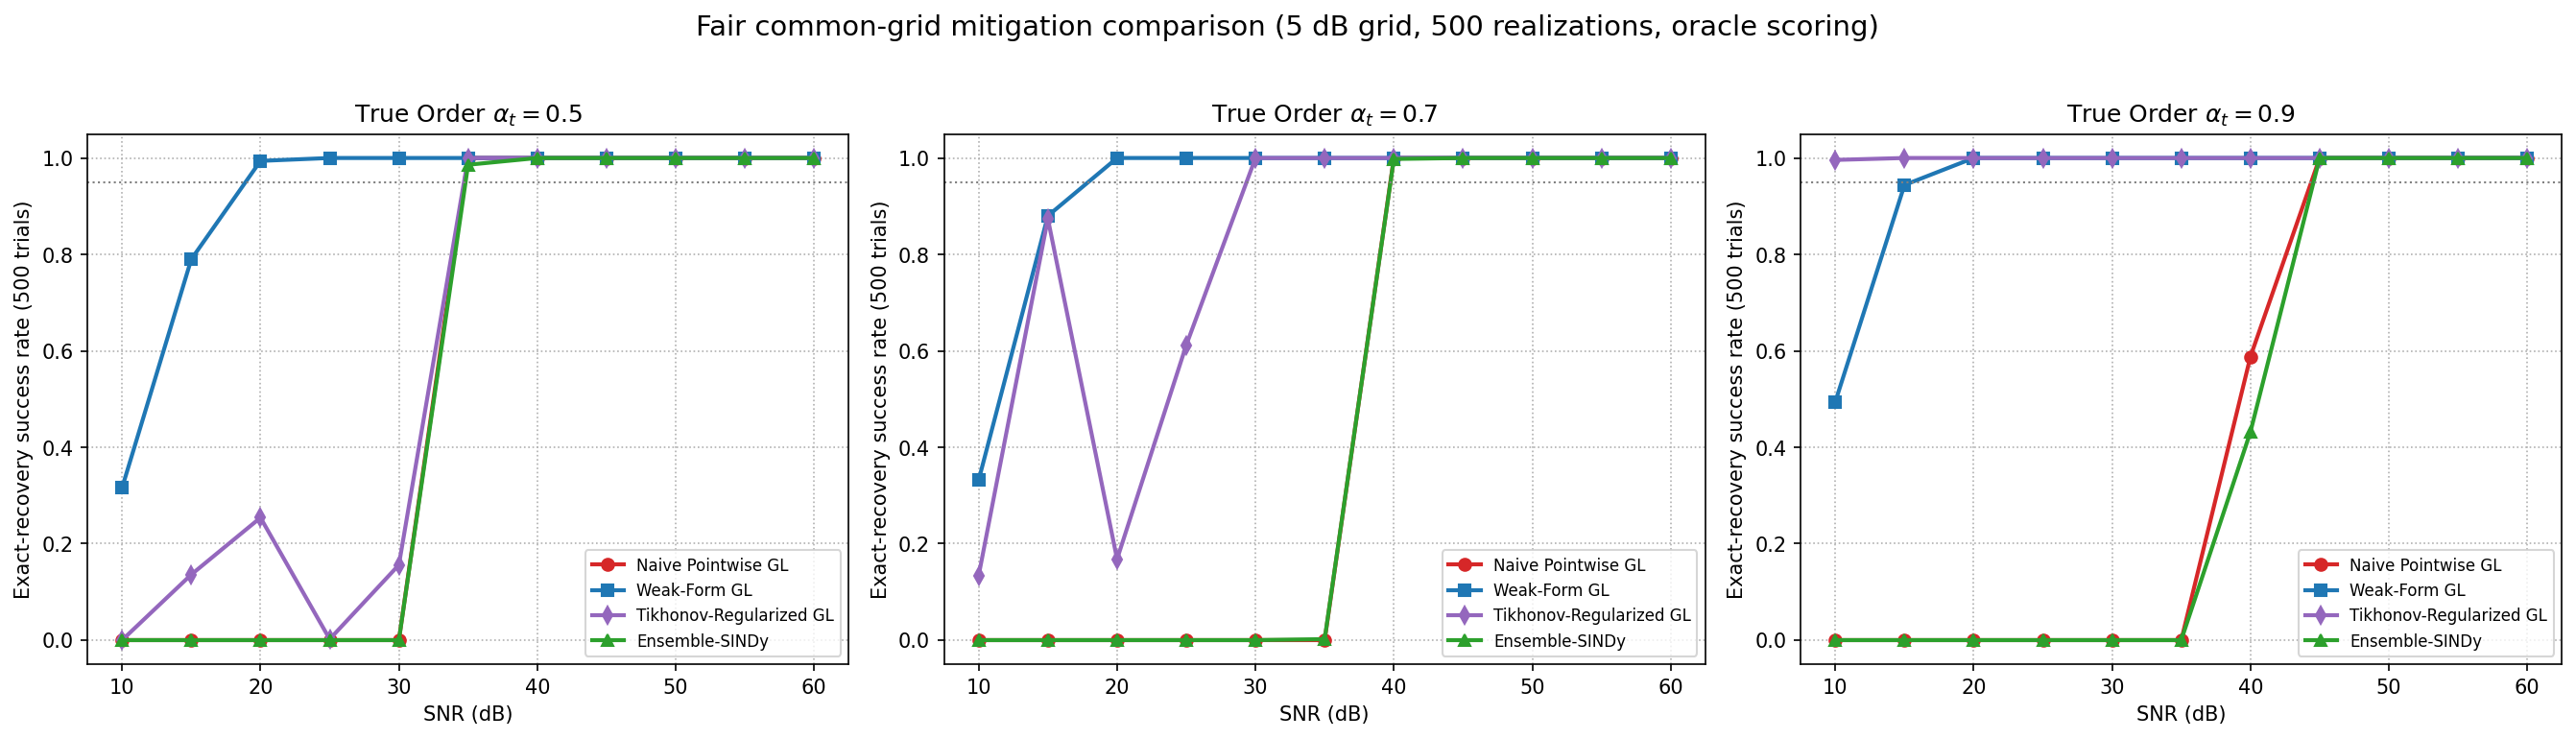
\includegraphics[width=0.9\textwidth]{../figures/mitigation_fairgrid.png}
\caption{Fair common-grid mitigation comparison: exact-recovery success rate (over 500 trials) versus SNR (dB) for all four methods---Naive Pointwise GL, Weak-Form GL, Tikhonov-regularized GL, and Ensemble-SINDy---across true fractional orders $\alpha_t \in \{0.5, 0.7, 0.9\}$, on the identical $5$ dB grid with identical seeds and oracle scoring. The dotted line marks the $95\%$ recovery criterion.}
\label{fig:mitigation_comparison}
\end{figure}

The comparison reveals that the weak-form formulation is the most robust \emph{general-purpose} remedy, though---under the fair comparison---it is not uniformly superior:
\begin{itemize}
  \item \textbf{Refutation of low-order memory tail hypothesis:} We previously conjectured that the slow decay of the memory kernel $t^{-\alpha}$ for low $\alpha$ prevents recovery of $\alpha_t=0.5$ under noise due to noise integration in the tail. However, our noise-amplification analysis shows that $A(0.5)$ is actually $56$ times smaller than $A(0.9)$. In agreement with this, the fine-grid Monte Carlo sweep demonstrates that the weak-form GL SINDy successfully recovers the differentiation order down to $20$ dB SNR for all true orders $\alpha_t \in \{0.5, 0.7, 0.9\}$ (with success rates of $99.4\%$, $100\%$, and $100\%$ at $20$ dB, respectively). Extending the weak-form sweep below the original $20$ dB floor establishes a lower fail edge at $15$ dB, so the three thresholds collapse to a common $[15\text{ dB}, 20\text{ dB}]$ bracket---indistinguishable at the $5$ dB grid resolution rather than provably order-independent. The $15$ dB fail-edge rates are $79.0\%$ ($\alpha_t=0.5$), $88.0\%$ ($\alpha_t=0.7$), and $94.4\%$ ($\alpha_t=0.9$); with Wilson $95\%$ score intervals of $[75.2,82.3]\%$, $[84.9,90.6]\%$, and $[92.0,96.1]\%$ respectively, the low-order edges are robustly below the $95\%$ criterion, but the $\alpha_t=0.9$ edge is \emph{criterion-fragile}---its interval straddles $95\%$---so whether that cell counts as ``fail'' depends on the noise realizations to within the confidence interval.
  \item \textbf{High-order selection bias at the noise floor:} The apparent recoveries below $15$ dB are not symmetric chance grid-snaps (which would give the uniform $1/9\approx 11\%$ per candidate). Instead, at the noise floor the selector concentrates its choice on \emph{high} candidate orders, so a high \emph{true} order inherits an inflated apparent success: at $0$ dB, $96\%$ of the weak-form selections for $\alpha_t=0.9$ fall in the high band $\hat\alpha\ge0.8$ (modal $\hat\alpha=0.9$), producing a $48.2\%$ ``recovery'' rate, whereas $\alpha_t=0.7$ yields $34.0\%$ and $\alpha_t=0.5$ only $0.4\%$ (modal $\hat\alpha=0.3$). The sub-15 dB ``successes'' are thus an order-dependent selection-bias artifact, not genuine recovery.
  \item \textbf{Order-Dependent Improvements:} The weak-form formulation yields a $15$ dB improvement for $\alpha_t=0.5$ ($[15\text{ dB}, 20\text{ dB}]$ vs $[30\text{ dB}, 35\text{ dB}]$), a $20$ dB improvement for $\alpha_t=0.7$ ($[15\text{ dB}, 20\text{ dB}]$ vs $[35\text{ dB}, 40\text{ dB}]$), and a $25$ dB improvement for $\alpha_t=0.9$ ($[15\text{ dB}, 20\text{ dB}]$ vs $[40\text{ dB}, 45\text{ dB}]$). By projecting the derivatives onto smooth compactly-supported test functions, the weak form bypasses the $h^{-2\alpha}$ noise amplification term that limits pointwise methods.
  \item \textbf{Ensemble-SINDy and Tikhonov Pre-smoothing:} On the fair common grid, bootstrapping (Ensemble-SINDy) provides essentially no improvement over naive pointwise GL ($[30,35]$/$[35,40]$/$[40,45]$ dB, identical to pointwise) because bagging pointwise estimates still inherits pointwise noise amplification. Tikhonov pre-smoothing is strongly order-dependent. With an \emph{SNR-tuned} $\lambda$ it is worse than weak-form at low order ($[30,35]$ dB at $\alpha_t=0.5$, $[25,30]$ dB at $\alpha_t=0.7$) but \emph{beats} weak-form at high order, recovering $\alpha_t=0.9$ down to $[{<}10,10]$ dB ($99.6\%$ at $10$ dB) where heavy smoothing preserves the large-amplitude high-order signal (its success curve is also non-monotone near threshold, e.g.\ $\alpha_t=0.7$: $87.4\%$ at $15$ dB dropping to $16.8\%$ at $20$ dB, making it less predictable than the weak form). That schedule is itself SNR-informed, so we re-ran Tikhonov with two $\lambda$ rules that use no SNR knowledge (Table~\ref{tab:mitigation_comparison}): a per-realization GCV selection and a fixed $\lambda=28.2$. Roughly half of the high-order advantage is SNR-tuning---under GCV the $\alpha_t=0.9$ bracket relaxes from $[{<}10,10]$ to $[10,15]$ dB, still one grid step better than weak-form's $[15,20]$, but GCV is markedly \emph{worse} at low order ($[30,35]$ dB at $\alpha_t\in\{0.5,0.7\}$) because with no noise prior it under-smooths the small-amplitude low-order target; the fixed $\lambda$ instead \emph{ties} weak-form's uniform $[15,20]$ at every order. Thus, under oracle scoring, weak-form and fixed-$\lambda$ Tikhonov \emph{tie} as the two parameter-fixed (no-SNR-knowledge) methods that recover every order at $\le 20$ dB, while Tikhonov's high-order edge is genuine but order-specific and shrinks to one grid step (GCV) or a tie (fixed $\lambda$) once SNR knowledge is removed. The tie itself is an oracle artifact: re-scored under the deployment-realistic rule of Section~\ref{sec:realistic}, Tikhonov loses to weak-form at every order.
\end{itemize}

\subsection{Deployment-Realistic Order Selection}
\label{sec:realistic}
All brackets above are produced by an oracle criterion that scores candidates against the clean ground-truth derivative evaluated at the true order---side information unavailable in practice. To measure what is actually deployable, we re-run the entire pointwise and weak-form sweep (same $5$ dB grid, same $500$ realizations, same seeds, same candidate grid and exact-match criterion) under a single principled rule that uses only the noisy data: held-out $R^2$ on a noisy validation split, where each candidate's model is fit on the noisy training split and scored on the noisy validation split against \emph{that candidate's own} GL derivative (pointwise) or weak projection (weak-form) of the noisy validation data. This is the literal deployable analog of the oracle rule (clean trajectory $\to$ noisy data, true order $\to$ candidate order). Because fixed-$\lambda$ Tikhonov ties weak-form under oracle scoring, we also re-score Tikhonov under the identical rule applied to the Tikhonov-smoothed noisy data (smooth-then-select), for both no-SNR-knowledge $\lambda$ rules---fixed $\lambda = 28.2$ and per-realization GCV---on the same $5$ dB spacing ($\{20,\dots,90\}$ dB) with the same realizations and seeds. The rule was fixed in advance; we report its output as-is.

The consequences are substantial (Table~\ref{tab:realistic}). First, every method degrades: the pointwise succeed edges move from $35/40/45$ dB to $60/70/65$ dB and the weak-form edges from a uniform $20$ dB to $45/45/35$ dB ($15$--$30$ dB each), while Tikhonov degrades hardest---with the fixed $\lambda=28.2$ that ties weak-form under the oracle, the succeed edges move from a uniform $20$ dB to $50/45$ dB for $\alpha_t=0.7/0.9$ and to \emph{no stable recovery anywhere in the grid} ($\le 90$ dB) for $\alpha_t=0.5$; with GCV $\lambda$, from $35/35/15$ dB to $55/65/65$ dB. The oracle brackets are therefore genuine identifiability ceilings, not deployable thresholds. Second, the clean monotonic-in-$\alpha$ ordering does not survive: realistic pointwise selection is non-monotone in $\alpha$ ($\alpha_t=0.7$ becomes the hardest, not $\alpha_t=0.9$), i.e.\ roughly flat at $55$--$70$ dB, while realistic weak-form selection \emph{inverts}, with the high-order case $\alpha_t=0.9$ now the easiest ($[30,35]$ dB) and the low-order case the hardest; realistic fixed-$\lambda$ Tikhonov likewise finds high order easiest (its low-order case fails outright), whereas the GCV variant is easiest at low order ($[50,55]$ vs $[60,65]$ dB). The low-$\alpha$-easiest ordering predicted by $A(\alpha)$ is thus specific to oracle scoring. Third, the weak form's advantage is now \emph{tested} against every mitigation rather than asserted: realistic weak-form ($35$--$45$ dB) beats realistic pointwise ($60$--$70$ dB) by $15$--$30$ dB and beats both realistic Tikhonov variants at every order ($5$--$10$ dB ahead of the better Tikhonov variant at each order; the worse variant trails by $20$--$30$ dB or fails outright), so the weak form remains the only deployable selector among the methods tested. Tikhonov's oracle tie does not transfer because what survives smoothing at high SNR is the smoothing bias itself: at $90$ dB the fixed-$\lambda$ pipeline selects $\hat\alpha=0.7$ for true $\alpha_t=0.5$ in $500/500$ realizations, confining its $\alpha_t=0.5$ success to a transient $[45,55]$ dB window that collapses again above $60$ dB. We also note that the realistic weak-form success curves are non-monotone (criterion-fragile) near their thresholds, consistent with the noise-floor analysis above.

\begin{table}[htbp]
\centering
\caption{Oracle (identifiability-ceiling) versus deployment-realistic recovery brackets $[$Fail, Succeed$]$ on the primary system, same $5$ dB grid spacing / $500$ realizations / seeds. The realistic rule uses only noisy data (held-out noisy $R^2$ with candidate-consistent targets); for Tikhonov it is applied to the pre-smoothed noisy data (smooth-then-select) with $\lambda$ chosen without SNR knowledge (fixed $\lambda = 28.2$ or per-realization GCV). A dagger ($\dagger$) marks a non-monotone success curve near threshold; the bracket uses the stable succeed edge. ``None'' means no stable recovery anywhere in the $\{20,\dots,90\}$ dB grid.}
\label{tab:realistic}
\begin{tabular}{lcccccc}
\toprule
& \multicolumn{2}{c}{$\alpha_t = 0.5$} & \multicolumn{2}{c}{$\alpha_t = 0.7$} & \multicolumn{2}{c}{$\alpha_t = 0.9$} \\
\cmidrule(lr){2-3}\cmidrule(lr){4-5}\cmidrule(lr){6-7}
Method & Oracle & Realistic & Oracle & Realistic & Oracle & Realistic \\
\midrule
Pointwise GL & [30, 35] & [55, 60] & [35, 40] & [65, 70] & [40, 45] & [60, 65] \\
Weak-Form GL & [15, 20] & [40, 45]$^\dagger$ & [15, 20] & [40, 45] & [15, 20] & [30, 35] \\
Tikhonov (fixed $\lambda$) & [15, 20] & None & [15, 20] & [45, 50] & [15, 20] & [40, 45] \\
Tikhonov (GCV $\lambda$) & [30, 35] & [50, 55] & [30, 35] & [60, 65] & [10, 15] & [60, 65] \\
\bottomrule
\end{tabular}
\end{table}

\subsection{Generality: An Independent Fractional Benchmark}
\label{sec:benchmark}
All results so far rest on a single primary system. To test generality we repeat the core analysis on an independent canonical fractional benchmark with a known ground-truth order: the fractional Van der Pol oscillator, $D^\alpha_t x = y$, $D^\alpha_t y = \mu(1-x^2)y - x$ with $\mu = 2.0$, integrated by the same explicit Gr\"unwald-Letnikov scheme and identified with a degree-3 polynomial library in $(x,y)$. Its sustained limit cycle provides a persistently excited, qualitatively different test bed from the primary relaxation system.

Both core findings reproduce. (i) Two-sided identifiability holds on clean data: the pipeline recovers the exact order for $\alpha_t \in \{0.5, 0.7, 0.9\}$ (sensitivity) and selects the integer order over all fractional candidates at $\alpha_t = 1.0$ (specificity), under both pointwise and weak-form scoring. (ii) The noise-amplification factor $A(\alpha)$ again rises monotonically with $\alpha$ (from $A(0.3)\approx 10.1$ to $A(0.9)\approx 1383.5$ and $A(1.0)\approx 3192.0$ at this system's time step), and the pointwise oracle recovery threshold again \emph{rises monotonically with the order}---succeed edges of $15$, $20$, and $25$ dB for $\alpha_t = 0.5, 0.7, 0.9$---reproducing the low-$\alpha$-easiest ordering of the primary system (whose corresponding edges were $35/40/45$ dB; the absolute SNRs are lower here because the limit-cycle signal is richer). (iii) The weak-form rescue reproduces: weak-form scoring lowers or ties the pointwise threshold at every order ($\alpha_t=0.7$: $[5,10]$ vs $[15,20]$ dB; $\alpha_t=0.9$: $[15,20]$ vs $[20,25]$ dB; $\alpha_t=0.5$: tie at $[10,15]$ dB). The magnitude of the weak-form advantage is smaller on this system than on the primary one---i.e.\ the \emph{size} of the rescue is system-dependent---but its \emph{direction} is not. The same oracle-versus-deployment caveat of Section~\ref{sec:realistic} applies to these benchmark brackets.

\subsection{Stability and Lyapunov Exponent Estimation Cautions}
We conduct chaos diagnostics on the ground-truth integer-order system. The variational equations integrated via Benettin's method yield an asymptotically negative maximum Lyapunov exponent:
\begin{equation}
\lambda_{\max} = -0.073362.
\end{equation}
This negative value proves that the model settles to a stable, non-chaotic steady state, as shown in the convergence curve of Fig.~\ref{fig:diagnostics_caution}(a).

\begin{figure}[htbp]
\centering
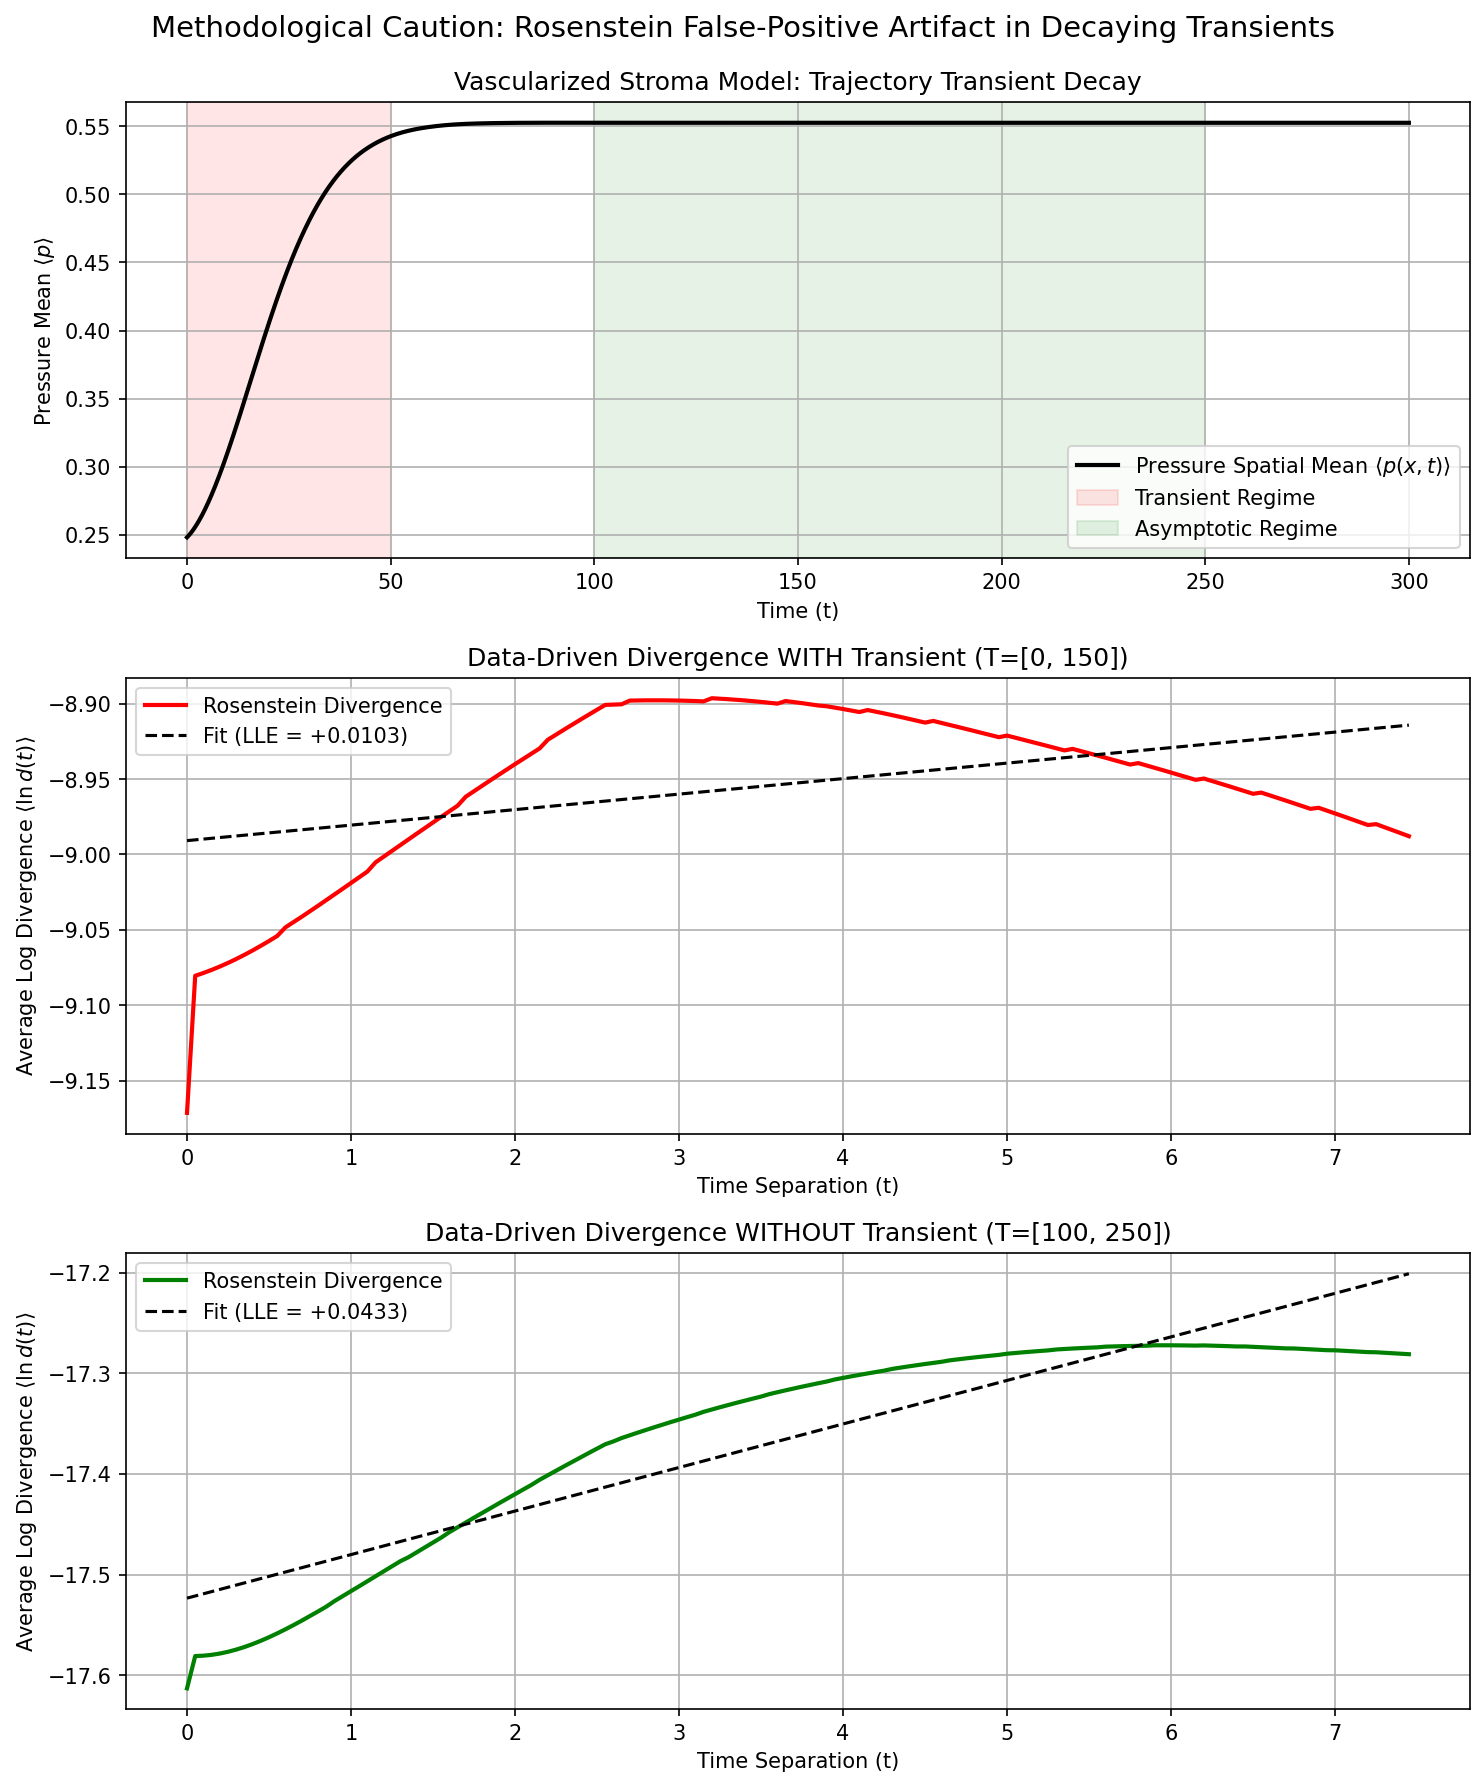
\includegraphics[width=0.85\textwidth]{../figures/diagnostics_caution.png}
\caption{Lyapunov exponent diagnostic curves. (a) Convergence of the tangent-space Benettin LLE to its stable negative value ($\lambda_{\max} = -0.073362$). (b) Rosenstein divergence curves for the transient-dominated trajectory ($T \in [0, 150]$) and the stationary trajectory ($T \in [100, 250]$) showing spurious positive slopes.}
\label{fig:diagnostics_caution}
\end{figure}

However, the data-driven Rosenstein estimator yields spurious positive exponents across all scenarios:
\begin{itemize}
  \item \textbf{Baseline (Full Time Series)}: $\text{LLE} = +0.018965$.
  \item \textbf{Transient-dominated ($T \in [0, 150]$)}: $\text{LLE} = +0.010285$.
  \item \textbf{Stationary-dominated ($T \in [100, 250]$)}: $\text{LLE} = +0.043278$.
\end{itemize}

These false positives highlight two distinct methodological failure modes of purely data-driven chaos estimators:
\begin{enumerate}
  \item \textbf{Transient Artifact}: On decaying transients, trajectories contract toward the fixed point. Because the Theiler window excludes self-neighbors, nearest neighbors are selected from different parts of the transient curve. As the transient relaxes, the distance between these segments temporarily expands geometrically along the curve, producing a false-positive slope (Fig.~\ref{fig:diagnostics_caution}(b), transient curve).
  \item \textbf{Stationary Noise Artifact}: Once the trajectory reaches the fixed point, the signal drops to solver precision limits ($10^{-8}$) or the noise floor. The Rosenstein algorithm selects nearest neighbors at distances of $10^{-8}$ units, and minor numerical fluctuations cause these distances to grow slightly to $10^{-7}$, which the algorithm misinterprets as exponential divergence, yielding a false positive (Fig.~\ref{fig:diagnostics_caution}(b), stationary curve).
\end{enumerate}
In contrast, tangent-space integration (Benettin) tracks the growth of analytic perturbations, which can contract indefinitely without saturation or geometric distortion, correctly yielding a negative exponent.

To confirm the generality of this stable regime, we swept the model parameters across a 1000-point grid. Every parameter combination evaluated is linearly stable. The maximum growth rate occurs at the corner of the envelope ($\rho = 0.1, \gamma_n = 5.0, D_n = 0.001$), yielding $\max \text{Re}(\lambda) = -0.001726$ (the stability map is shown in Fig.~\ref{fig:stability_map}). To ensure this soft boundary did not hide adjacent instabilities, we evaluated points just past the corner (Table~\ref{tab:stability_corner}), confirming that stability is preserved.

\begin{table}[htbp]
\centering
\caption{Leading eigenvalue $\text{Re}(\lambda)$ at parameter points past the corner of the sweep envelope.}
\label{tab:stability_corner}
\begin{tabular}{cccc}
\toprule
Point & Parameter Changes & Leading $\text{Re}(\lambda)$ & Status \\
\midrule
A & Lower growth: $\rho = 0.05, \gamma_n = 5.0, D_n = 0.001$ & -0.000860 & Stable \\
B & Higher regression: $\rho = 0.1, \gamma_n = 6.0, D_n = 0.001$ & -0.001437 & Stable \\
C & Lower diffusion: $\rho = 0.1, \gamma_n = 5.0, D_n = 0.0005$ & -0.001726 & Stable \\
D & Extrapolated corner: $\rho = 0.05, \gamma_n = 6.0, D_n = 0.0005$ & -0.000716 & Stable \\
\bottomrule
\end{tabular}
\end{table}

\begin{figure}[htbp]
\centering
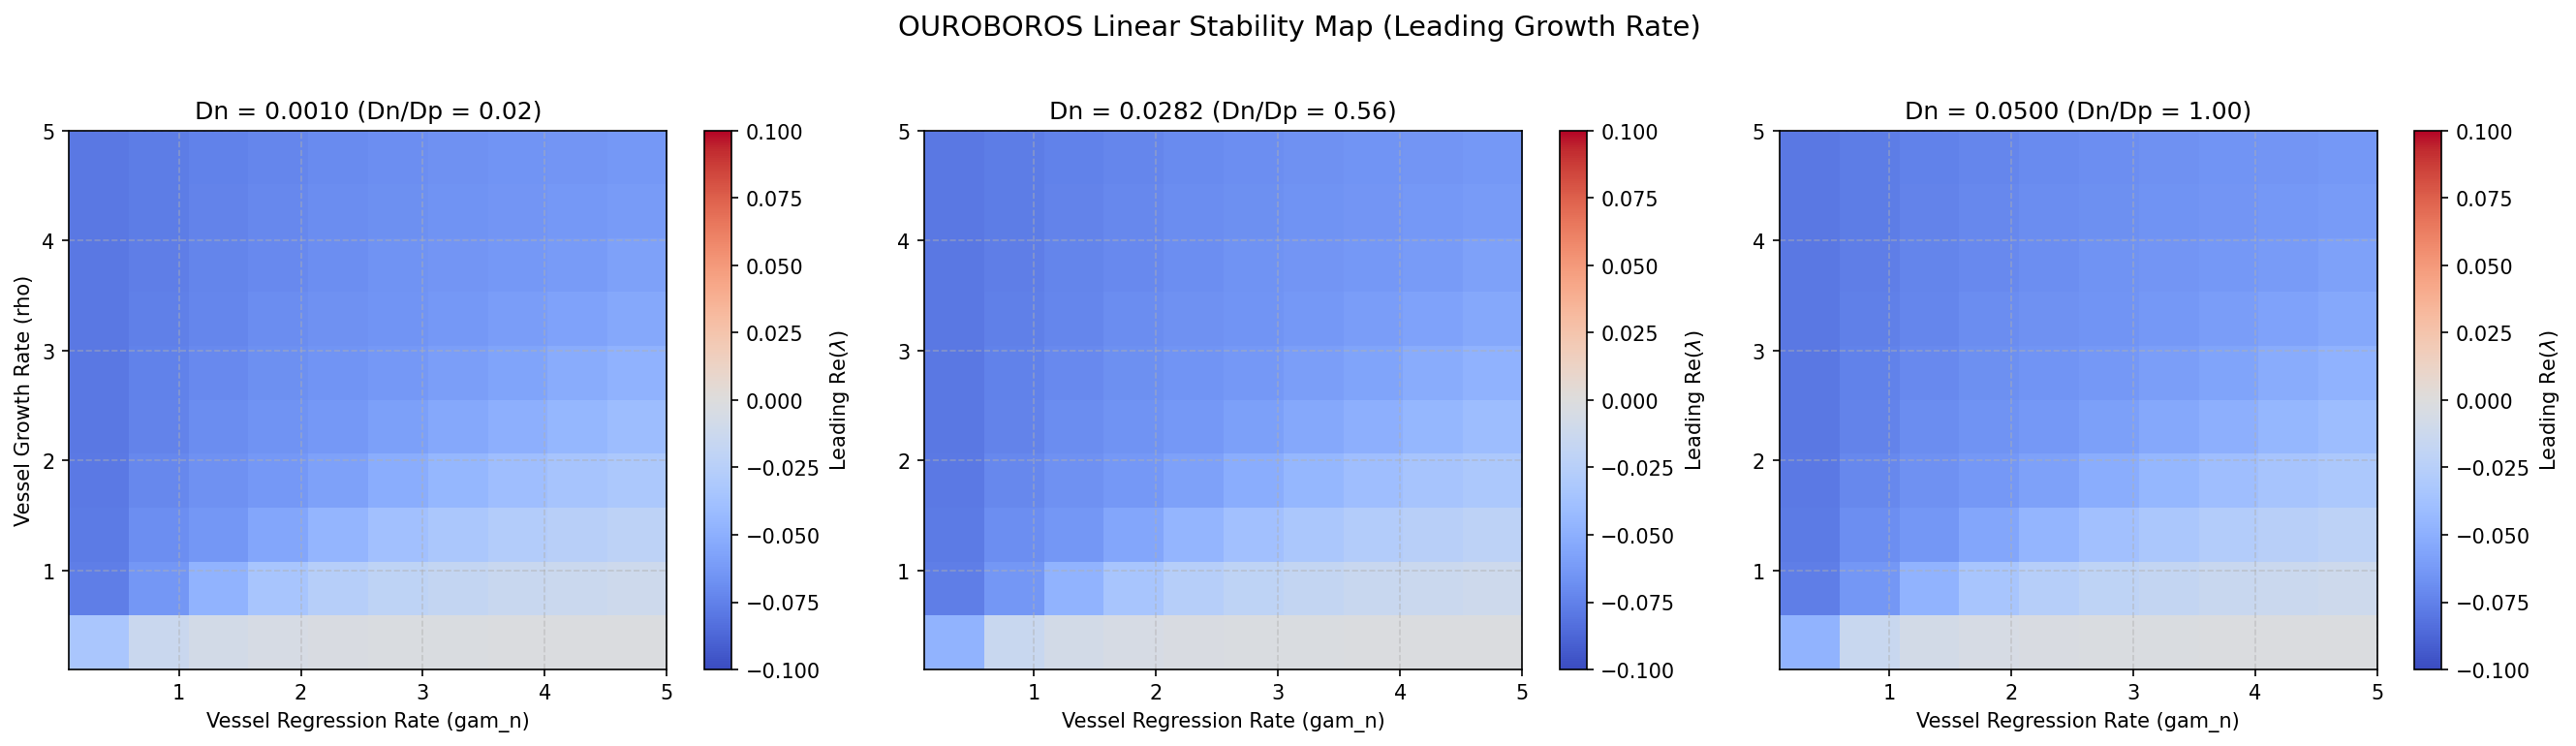
\includegraphics[width=0.9\textwidth]{../figures/stability_map.png}
\caption{Linear dispersion stability maps. The plot maps the maximum eigenvalue growth rate $\text{Re}(\lambda)$ across the parameter space grid ($\rho$, $\gamma_n$, $D_n$), indicating global stability ($\text{Re}(\lambda) < 0$) throughout.}
\label{fig:stability_map}
\end{figure}

\section{Discussion and Related Work}
Data-driven discovery of fractional differential equations is an active research area. In particular, the sparse identification of fractional chaotic systems from time-domain data (SIFCS) has been proposed by Zhang et al. \cite{zhang2024sifcs}, utilizing joint iterative thresholding over the fractional order and claiming robust identification of chaotic dynamics. Concurrently, data-driven frameworks for discovering fractional differential equations (FDEs) in complex systems have been introduced, such as the deep neural network and Gauss-Jacobi quadrature method by Yu et al. \cite{yu2025fde} and related methods \cite{wang2024fracid} to reconstruct and identify FDE structures. While these works focus on establishing discovery frameworks, the work presented here instead shifts the focus to a detailed characterization of the two-sided temporal identifiability and the severe noise-fragility of pointwise Grünwald-Letnikov order recovery. Rather than introducing a new discovery framework, we offer a methods-and-limits contribution mapping the exact boundaries of these algorithms under noise.

It is worth delimiting precisely what is new here versus what is applied from established methods. The headline contribution is a \emph{cautionary characterization}---a map of where data-driven fractional order selection is identifiable and where it is not---rather than a new noise-robust recovery method; the weak form is the best available mitigation, but the paper's result is the boundary it does not cross, not a deployable rescue. Our novel contributions are specific to the fractional-order setting: (i) the closed-form Gr\"unwald-Letnikov noise-amplification factor $A(\alpha) = h^{-2\alpha}\|w(\alpha)\|_2^2$ and the resulting, counter-intuitive monotone-in-$\alpha$ difficulty ordering (high orders are \emph{harder} to recover under noise, opposite to the memory-tail intuition); (ii) the two-sided (specificity and sensitivity) temporal identifiability characterization for fractional order selection, including its reproduction on an independent benchmark; and (iii) the distinction between the oracle identifiability ceiling and the deployment-realistic bracket, which shows the published ceilings are not directly deployable. The weak-form SINDy machinery we use as the remedy is, by contrast, an established, general principle that we apply---not invent---in the fractional setting, as detailed next.

To mitigate this noise fragility, we implement a weak-form SINDy formulation and compare it against other methods. The weak-form (or integral-form) formulation is an established principle in the sparse identification literature, originally introduced by Schaeffer and McCalla \cite{schaeffer2017integral} for model selection via integral terms and extended to partial differential equations by Messenger and Bortz \cite{messenger2021wsindy}. Similarly, ensemble bagging methods have been proposed by Fasel et al. \cite{fasel2022ensemble} to improve sparse model discovery under high-noise limits. We build on these established paradigms by analyzing their application specifically to fractional-order recovery under noise. We find that, on a fair common grid, the weak-form formulation is the most robust \emph{general-purpose} remedy under oracle scoring: it recovers differentiation orders down to a common $[15\text{ dB}, 20\text{ dB}]$ bracket for all true orders $\alpha_t \in \{0.5, 0.7, 0.9\}$ (indistinguishable at the $5$ dB grid resolution rather than provably order-independent) and is one of only two methods---the other being fixed-$\lambda$ Tikhonov, which ties it under oracle scoring---that help at low order. It is not, however, universally superior: Tikhonov pre-smoothing surpasses it at high order ($\alpha_t = 0.9$, recovering to $[{<}10,10]$ dB), where heavy smoothing preserves the large-amplitude high-order signal. That advantage is, however, largely an artifact of SNR-tuned $\lambda$: re-running Tikhonov with $\lambda$ rules that use no SNR knowledge shrinks the high-order edge to a single grid step under a data-driven (GCV) $\lambda$ ($[10,15]$ vs weak-form $[15,20]$ dB, while GCV is far worse at low order) and to a tie under a fixed $\lambda$. Ensemble bagging gives no improvement over naive pointwise GL. This refutes our earlier conjecture that low-order fractional recovery is fundamentally precluded by noise accumulation in the memory tail---a hypothesis that the noise-amplification analysis independently overturns, since $A(\alpha)$ in fact \emph{rises} with $\alpha$---showing instead that the weak form suppresses the dominant $h^{-2\alpha}$ noise amplification that limits pointwise methods. We caution that all of these brackets are oracle (clean-derivative) ceilings: under a deployment-realistic rule using only noisy data (Section~\ref{sec:realistic}) every method degrades by $15$ dB or more---Tikhonov most of all, its oracle tie with weak-form collapsing to a loss at every order---and the weak form, while remaining the best (and only) deployable option among those tested, no longer exhibits a clean monotone-in-$\alpha$ ordering. The qualitative picture---monotone $A(\alpha)$, two-sided clean identifiability, and a weak-form rescue---reproduces on an independent fractional Van der Pol benchmark (Section~\ref{sec:benchmark}), supporting its generality beyond the single primary system. We caution, nonetheless, that both test beds---the three-field relaxation system and the two-state Van der Pol oscillator---are low-dimensional; our case for generality rests on the dimension-agnostic noise-amplification mechanism (the $h^{-2\alpha}$ factor in $A(\alpha)$ depends only on the time step and order, not the state dimension) rather than on a high-dimensional demonstration. Extending this characterization to higher-dimensional and real measured systems, and constructing a genuinely deployable noise-robust order selector, are deliberately left as future work---we make neither claim here.

Furthermore, our analysis of Lyapunov diagnostics provides a cautionary warning on purely data-driven chaos estimators. The false-positive chaos detected by the Rosenstein algorithm \cite{rosenstein1993practical} is consistent with the classic critiques by Kantz \cite{kantz1994robust} and Hegger et al. \cite{hegger1999practical}, who noted that data-driven LLE algorithms are highly sensitive to transient lengths, embedding parameters, and noise floors. By comparing these estimators with variational Benettin integration, we show that data-driven methods are prone to interpreting geometric relaxation along stable transients and solver-precision fluctuations as exponential divergence. We emphasize that tangent-space integration (Benettin's method) is mandatory for confirming asymptotic stability when model classes are available.

This Lyapunov caution is not a separate aside but a second instance of the paper's unifying thread: purely data-driven diagnostics of nonlinear dynamics are fragile and can manufacture confident artifacts---an order that rails to the candidate floor or snaps to a high-order bias under noise in the identification setting, and a spurious positive Lyapunov exponent on a provably stable system in the chaos-diagnostic setting. In both cases the remedy is the same: anchor the data-driven estimate to a model-based computation (the weak-form integral operator and the $A(\alpha)$ variance formula for identification; the variational tangent-space integration for stability). Where a model class is available, such model-based diagnostics are not optional refinements but the only reliable arbiters.

\subsection{The Circularity Boundary and Claim Constraints}
To prevent scientific overreach when analyzing mathematical models of biological systems, we establish the boundary of defensible claims in Table~\ref{tab:claims}. 

\begin{table}[htbp]
\centering
\caption{Summary of defensible claims versus invalid biological claims.}
\label{tab:claims}
\begin{tabular}{p{7.5cm}p{7.5cm}}
\toprule
We CAN Defensibly Claim & We CANNOT Claim (Circularity/Scientific Violation) \\
\midrule
1. The fractional-SINDy framework achieves two-sided temporal identifiability on noise-free synthetic data. & 1. Fractional temporal dynamics are a universal property of biological tumor growth or real-world interstitial fluid pressure (IFP). \\
2. Purely data-driven Lyapunov estimators (e.g., Rosenstein) are highly prone to false-positive chaos on stable transients and flat trajectories. & 2. Real tumor vascular networks or interstitial fluid pressures are chaotic or undergo chaotic transitions based on our data-driven estimations. \\
3. Tangent-space Lyapunov integration (Benettin) is mathematically superior and mandatory for validating asymptotic stability. & 3. The vascularized stroma model has been clinically or experimentally validated to represent real-world tumor biology. \\
4. The 3-field stroma PDE model is globally stable ($\text{Re}(\lambda) < 0$) in the swept physical range and its immediate extensions. & 4. Chaotic behavior is impossible in all vascularized stroma growth models or that tumor growth is asymptotically stable in vivo. \\
\bottomrule
\end{tabular}
\end{table}

Without direct, high-frequency in vivo measurements of tumor IFP and oxygenation, independent calibration of physical parameters ($D_p$, $D_c$, $D_n$), and experimental validation of coupling terms ($-\gamma_n n p$), any claims must remain strictly confined to the mathematical model class and the recovery pipeline.

\section{Conclusion}
This study evaluated the identifiability, stability, and noise fragility of data-driven modeling pipelines on a vascularized stroma reaction-diffusion model. While fractional SINDy displays clean sensitivity and specificity in the noise-free limit, it is practically fragile under realistic noise. Under oracle scoring (against the clean ground-truth derivative), the weak-form GL SINDy is the most effective of the mitigations tested: it extends temporal order recovery down to a common bracket of $[15\text{ dB}, 20\text{ dB}]$ for all three orders $\alpha_t \in \{0.5, 0.7, 0.9\}$ (indistinguishable at the $5$ dB grid resolution), a $15$--$25$ dB improvement over naive pointwise GL, whose recovery threshold rises monotonically with the order---breaking down at brackets of $[30\text{ dB}, 35\text{ dB}]$, $[35\text{ dB}, 40\text{ dB}]$, and $[40\text{ dB}, 45\text{ dB}]$ for $\alpha_t = 0.5$, $0.7$, and $0.9$. We are careful to frame these as identifiability ceilings, not a usable recovery guarantee: under a deployment-realistic selection rule that uses only noisy data, every method degrades by $15$ dB or more and the monotone-in-$\alpha$ ordering does not survive, though the weak form remains the only deployable selector---a claim we test directly rather than assume: Tikhonov, re-scored under the identical realistic rule, loses to weak-form at every order---albeit a modest one; and on a fair common grid Tikhonov pre-smoothing surpasses the weak form at high order only when its $\lambda$ is SNR-tuned---without SNR knowledge that edge shrinks to a single grid step (data-driven $\lambda$) or vanishes to a tie (fixed $\lambda$), and even that tie holds only under oracle scoring. These identifiability, amplification, and rescue findings reproduce on an independent fractional Van der Pol benchmark. Furthermore, we demonstrated that data-driven Lyapunov exponent estimators (e.g., Rosenstein) produce spurious positive exponents on stable transients and noise floors, making analytical tangent-space integration (Benettin) mandatory for reliable stability characterization---the same lesson, in a different guise, that data-driven diagnostics require model-based anchoring. For practitioners, the operative lesson is that a clean-data identifiability bracket is an upper bound, not an operating point: data-driven fractional order selection should be treated as unreliable unless anchored to a model-based diagnostic---the $A(\alpha)$ variance formula or weak-form projection for identification, and variational tangent-space integration for stability.

\section*{Data and Code Availability}
The simulation codes, data generation scripts, and plotting routines developed for this study are available on GitHub at \url{https://github.com/akarlin3/projOuroboros} and will be archived on Zenodo under DOI: \href{https://doi.org/\zenododoi}{\texttt{\zenododoi}}.

\section*{Funding}
This research received no specific grant from funding agencies in the public, commercial, or not-for-profit sectors.

\section*{Declaration of Generative AI and AI-assisted technologies in the writing process}
During the preparation of this work the author used Claude (Anthropic) to assist with drafting and editing the manuscript text and with developing and debugging the analysis and figure-generation code. After using this tool, the author reviewed, verified, and edited all content and results and takes full responsibility for the content of the publication.

\bibliographystyle{elsarticle-num}
\bibliography{refs.bib}

\end{document}
